%% LyX 2.1.4 created this file.  For more info, see http://www.lyx.org/.
%% Do not edit unless you really know what you are doing.
\documentclass[english]{article}
\usepackage{charter}
\renewcommand{\familydefault}{\rmdefault}
\usepackage[T1]{fontenc}
\usepackage[latin9]{inputenc}
\usepackage{fancyhdr}
\pagestyle{fancy}
\usepackage{color}
\usepackage{babel}
\usepackage{array}
\usepackage{longtable}
\usepackage{graphicx}
\usepackage{setspace}
\onehalfspacing
\usepackage[unicode=true,pdfusetitle,
 bookmarks=true,bookmarksnumbered=false,bookmarksopen=false,
 breaklinks=false,pdfborder={0 0 0},backref=false,colorlinks=false]
 {hyperref}
\usepackage{breakurl}

\makeatletter

%%%%%%%%%%%%%%%%%%%%%%%%%%%%%% LyX specific LaTeX commands.
%% Because html converters don't know tabularnewline
\providecommand{\tabularnewline}{\\}

%%%%%%%%%%%%%%%%%%%%%%%%%%%%%% User specified LaTeX commands.
\usepackage{babel}
\usepackage{babel}
\usepackage{babel}
\usepackage{babel}






\usepackage{listings}
\renewcommand{\lstlistingname}{Listing}





\usepackage{listings}
\renewcommand{\lstlistingname}{Listing}



\usepackage{listings}
\renewcommand{\lstlistingname}{Listing}

\makeatother

\usepackage{listings}
\renewcommand{\lstlistingname}{Listing}

\begin{document}

\title{Requirements Analysis and Specification Document}

\maketitle
\begin{center}

\includegraphics[height=0.3\textheight]{polimiLogo}
\par\end{center}

\begin{center}
Daniele Grattarola (Mat. 853101)
\par\end{center}

\begin{center}
Ilyas Inajjar (Mat. 790009) 
\par\end{center}

\begin{center}
Andrea Lui (Mat. 850680)
\par\end{center}


\title{\pagebreak{}}

\tableofcontents{}

\pagebreak{}


\section{Introduction}


\subsection{Purpose}

The presented document is the Requirements Analysis and Specification
document (RASD) for the MyTaxiService platform project.

The main purpose of this document is to analyze the problems that
the new system is to solve and the customer's necessities, to identify
use cases and actors, to describe the functional and non-functional
requirements of the platform along with existing constraints, and
to propose an in-depth specification of the system before moving on
to the more concrete design phase.

This document is intended for stakeholders, software engineers, and
programmers and is to be used as reference throughout the whole development
of the system. Each phase of the project must be brought on with this
document in mind, and any implementation of the system must be clearly
designed to reflect the specifications presented here.

The secondary audience for this document includes system maintainers
and developers who wish to integrate the platform's services within
their own software.


\subsection{Scope}

The aim of this project is to create the MyTaxiService platform, a
web based information system to manage the taxi service of Pallet
Town.

The purpose of the platform is: 
\begin{enumerate}
\item To provide users with a web application and a mobile application,
with which to easily make use of the town's taxi service. 
\item To provide taxi drivers with a mobile application, with which to manage
customers' requests (submitted through the above mentioned systems) 
\end{enumerate}
In short, the platform is to be an integrated infrastructure to manage
the initial interaction between customers and taxi drivers, to aid
the former in requesting a taxi ride, and to enable the latter in
managing such requests.

The platform will therefore be used exclusively to support the town's
taxi service, and is aimed at making the taxi request process much
efficient by reducing overall costs, communication overhead and potential
requests overloads.

The platform will implement all necessary functions on both the users'
side and the drivers', while keeping the two aspects separate and
unaware of each other. It will also be given a particular focus to
the storage of user data, in order to maximize privacy and security,
and to the extensibility of the system, in order to make the platform
flexible to potential changes in the requirements.


\subsection{Definitions, acronyms, and abbreviations \label{sub:Definitions,-acronyms,-and}}

Throughout this document, the following definitions will be applied
without further explanations: 
\begin{itemize}
\item \textbf{Platform}: the set of software applications and hardware infrastructure
that make up the MyTaxiService service; these include the back-end
server software, the web application and the mobile application used
by the customers, the mobile application used by the taxi drivers,
and all the necessary hardware needed to run the mentioned software
and any needed support software. 
\item \textbf{System}: any subset of software components of the platform. 
\item \textbf{Back-end}: the software run on the back-end server of the
platform which is used to handle the communication between the user
applications. The term also addresses all the necessary software components
that are needed to store data, perform calculations and manage the
hardware (e.g. an operating system). 
\item \textbf{Customer-side application}: software run on a personal device
which is used to send taxi requests to the system and to handle the
system's replies. It is designed to be used by customers (see below)
and can either be a mobile application (run on a smartphone or tablet)
or a web application (run on any personal device through an Internet
browser). 
\item \textbf{Taxi-side application}: software run on a personal device
which is used to manage taxi requests forwarded by the system and
to reply to the system with information on how to handle the requests.
It is designed to be used by taxi drivers (see below) and is a mobile
application (run on a smartphone or tablet). 
\item \textbf{User-side application}: the set of customer-side and taxi-side
applications 
\item \textbf{Taxi driver}: the owner of a taxi license in Pallet Town,
who uses the taxi-side application to interact with the platform. 
\item \textbf{Customer}: a person which intends to exploit the taxi service
of the town, and who uses the user-side applications to interact with
the platform. 
\item \textbf{User}: any customer or taxi driver who uses a user-side application. 
\end{itemize}
The following acronyms will also be used in place of the extended
form: 
\begin{itemize}
\item \textbf{RASD}: Requirement Analysis and Specification Document 
\item \textbf{CGI}: Common Gateway Interface 
\item \textbf{DBMS}: Data Base Management System 
\item \textbf{RTO}: Recovery Time Objective 
\item \textbf{RPO}: Recovery Point Objective 
\item \textbf{SOC}: System On a Chip 
\end{itemize}
The following convention will be used to refer to different items
in the document:
\begin{itemize}
\item \textbf{sec. / secs.}: section / sections
\item \textbf{req.}: requirement.
\end{itemize}
A typical use of the aforementioned abbreviation would be in the form
``element Xx, sec. x.x.x'' (e.g. \textit{req. 1, sec. 1.3} - if
this section contained a numbered requirement with index 1).

One last observation is to be done regarding the use of the singular
\textit{they}, which will be used to refer to single persons throughout
the whole document. 


\subsection{Overview}

The presented RASD is divided in sections and structured as follows: 
\begin{itemize}
\item \textbf{Section 1 - Introduction}: contains support information to
better understand the presented document and provides a brief introduction
of the project, with its scope and general goals. 
\item \textbf{Section 2 - Overall description}: contains a high level descriptions
of the platform to be created, with its functions, conceptual structure,
relations with the outside world and design constraints. 
\item \textbf{Section 3 - Requirements}: contains an in-depth description
of the platform's functional and non functional requirements, its
use cases and actors, and a software design guide for developers. 
\item \textbf{Section 4 - Alloy modeling}: contains a description of the
platform in the Alloy modeling language.
\item \textbf{Section 5 - Additional comments}: contains a summary of the
hours spent in producing the document. 
\end{itemize}

\section{Overall Description}


\subsection{Product perspective}

The platform aims at replacing the traditional means of communication
between taxi drivers and customers, and it is therefore designed as
a stand-alone entity that is able to operate with a minimum set of
dependencies towards external systems.


\subsubsection{Software interfaces \label{sub:Software-Interfaces}}
\begin{itemize}
\item \textbf{Google Maps API}: used in both the back-end and the taxi-side
applications, this free API is necessary to elaborate routes and display
maps. The system interacts with the API through standard GET requests.

\begin{itemize}
\item Mnemonic: map rendering and route elaboration 
\item Documentation: https://developers.google.com/maps/ 
\end{itemize}
\item \textbf{GPS}: this well known system is required by the mobile applications
to get information about the users' position. The interaction happens
through the standard GPS protocol provided by the OS of the users'
devices.

\begin{itemize}
\item Mnemonic: user position 
\item Documentation: refer to OS-specific documentation 
\end{itemize}
\item \textbf{Red Hat Enterprise Linux}: operating system run on the back-end
server.

\begin{itemize}
\item Mnemonics: back-end OS 
\item Documentation: https://access.redhat.com/documentation/en/red-hat-enterprise-linux/ 
\end{itemize}
\item \textbf{Apache WebServer}: software bundle run on the back-end, which
is used to allow interaction between the back-end system and the user-side
application. It is used to handle standard HTTP requests from the
customer-side web application and to provide CGI services to all the
user-side applications.

\begin{itemize}
\item Mnemonics: web-server 
\item Documentation: https://httpd.apache.org/docs/2.4/ 
\end{itemize}
\item \textbf{SQLite}: DBMS software run on the back-end, which is used
to store user data in a non-resource-intensive fashion.

\begin{itemize}
\item Mnemonics: DBMS 
\item Documentation: https://www.sqlite.org/docs.html 
\end{itemize}
\end{itemize}

\subsubsection{User interfaces\label{sub:User-interface}}

The platform must be accessible to users through three different interfaces,
which must be transparent to the back-end and must provide a unified
user experience. 
\begin{itemize}
\item[{{{{\textbf{{[}I1{]}}}}}}] \textbf{Customer web application}: standard dynamic website generated
with information associated to the user. It is accessible through
any standard web browser. 
\item[{{{{\textbf{{[}I2{]}}}}}}] \textbf{Customer-side mobile application}: mobile application developed
with proprietary graphical libraries in order to maintain the same
business identity throughout the different mobile OSs that the application
targets. 
\item[{{{{\textbf{{[}I3{]}}}}}}] \textbf{Taxi-side mobile application}: mobile application developed
with proprietary graphical libraries in order to maintain the same
business identity throughout the different mobile OSs that the application
targets. 
\end{itemize}

\subsubsection{Device support\label{sub:Device-support}}

The back-end system is designed to be run exclusively on usual x64
server hardware and may therefore require fine-tuning of its environment,
but needs to be flexible for hardware scaling (such as replication)
in order to ensure its longevity.

The user-side mobile applications, on the other hand, are designed
to be run on standard SOC architectures like the vast majority that
is found on smartphones and tablets, and take into account the differences
in the mobile operating systems that can be run on the SOC.

Finally, the customer-side web application does not have specific
device requirements, since it relies on a different level of abstraction
(web browser) which is not to be considered as a hardware interface.


\subsection{Product functions\label{sub:Product-functions}}

The fully developed platform should implement the following high level
functions. 
\begin{itemize}
\item \textbf{Customer-side application}:

\begin{enumerate}
\item[{{{{\textbf{{[}F1{]}}}}}}] Allow users to request a taxi. 
\item[{{{{\textbf{{[}F2{]}}}}}}] Allow users to manage their profile. 
\item[{{{{\textbf{{[}F3{]}}}}}}] Allow users to issue taxi reports. 
\end{enumerate}
\item \textbf{Taxi-side application}:

\begin{enumerate}
\item[{{{{\textbf{{[}F4{]}}}}}}] Allow users to manage incoming requests. 
\item[{{{{\textbf{{[}F5{]}}}}}}] Allow users to manage their profile. 
\item[{{{{\textbf{{[}F6{]}}}}}}] Allow users to issue customer reports. 
\item[{{{{\textbf{{[}F7{]}}}}}}] Allow users to report a technical problem. 
\end{enumerate}
\item \textbf{Generic platform functions: }

\begin{enumerate}
\item[{{{{\textbf{{[}F8{]}}}}}}] Manage user authentication processes. 
\item[{{{{\textbf{{[}F9{]}}}}}}] Manage taxi queues in the different zones of the town. 
\end{enumerate}
\end{itemize}

\subsection{Actors and related functionalities\label{sub:Actors-and-related}}

The platform may have different functional and non-functional requirements
based on the user that is interacting with it. Throughout this document,
the set of these different requirements has been referred to with
the terminology specified in sec. \ref{sub:Definitions,-acronyms,-and}
(e.g. taxi-side application, customer-side application, etc.).

This section, instead, is aimed at giving a high level description
of the platform based on the different actors that participate in
its use: 
\begin{itemize}
\item[{{{{\textbf{{[}A1{]}}}}}}] \textbf{\label{-Guest:-any} Guest}: any person who wishes to start
a session with the platform through one of the user-side applications.
A1 actors may:

\begin{itemize}
\item Register a profile into the platform 
\item Log into the platform 
\item Retrieve their password 
\end{itemize}

After completing a login, A1 actors may become either of the two following
types of actor.

\item[{{{{\textbf{{[}A2{]}}}}}}] \textbf{\label{-Customer:-a} Customer}: a person as defined in sec.
\ref{sub:Definitions,-acronyms,-and}. Based on what actions A2 completes,
they can be further specialized in:

\begin{itemize}
\item[{{{{\textbf{{[}A2.1{]}}}}}}] \textbf{\label{-Logged-in-Customer:} Logged-in Customer}: an A1
actor who logged in to the platform with a customer profile. A2.1
actors may:

\begin{itemize}
\item Issue a taxi request 
\item View and edit their profile 
\end{itemize}
\item[{{{{\textbf{{[}A2.2{]}}}}}}] \textbf{\label{-Passenger:-an} Passenger}: an A2.1 actor who issued
a taxi request. A2.2 actors may:

\begin{itemize}
\item Cancel or edit the issued taxi request 
\item Issue a taxi report 
\end{itemize}
\end{itemize}
\item[{{{{\textbf{{[}A3{]}}}}}}] \textbf{\label{-Taxi-driver:} Taxi driver}: a person as defined
in sec. \ref{sub:Definitions,-acronyms,-and}. A3 actors may:

\begin{itemize}
\item Handle (accept or refuse) a taxi request issued by an A2 actor. 
\item Edit their availability status 
\item Issue a customer report 
\item Report a technical problem 
\end{itemize}
\end{itemize}

\subsubsection{User characteristics}

Users do not need specific competences to use the app other than a
basic knowledge of web browsing (customers only) and of their mobile
operating system (both customers and taxi drivers).


\subsection{Constraints\label{sub:Constraints}}

The development of the platform will be limited by the following constraints
to which the system must be subject to. These are not listed as part
of the specific requirements of the platform because they stem from
circumstances beyond the designers' control, and are not directly
part of the customer's requests. 
\begin{enumerate}
\item[{{{{\textbf{{[}C1{]}}}}}}] \textbf{Privacy policy}: processing of user data, be it personal
or related to the use of the platform, is to be carried out according
to the national laws and the ways and means of said processing must
be clearly defined and available to the users at any time. 
\item[{{{{\textbf{{[}C2{]}}}}}}] \textbf{Taxi licenses}: the use of the taxi-side application and
the related access to the platform, is intended exclusively for taxi
drivers officially recognized by the town's appropriate taxi organizations. 
\item[{{{{\textbf{{[}C3{]}}}}}}] \textbf{Data integrity and data security}: users' personal data must
be stored according to specific standards that guarantee their integrity
and security. Further analysis of this constraint will be carried
out in sec. \ref{sub:Security-requirements}. 
\item[{{{{\textbf{{[}C4{]}}}}}}] \textbf{Legal waiver of responsibility}: due to the nature of the
platform's domain, the use of the platform can be associated to car
accidents and other related possible injuries; users are therefore
required to accept a legal disclaimer, in order to use the platform. 
\end{enumerate}

\subsection{Domain assumptions\label{sub:Domain-Assumptions}}

Some domain assumption have to be introduced in order to further define
the scope of the project, and to clearly state under which assumptions
the development should proceed in those areas that are not explicitly
covered by the initial customer's specification.

The assumptions are the following: 
\begin{enumerate}
\item[{{{{\textbf{{[}DA1{]}}}}}}] It is assumed that the user-side devices are capable of running the
intended user-side applications, according to the descriptions in
sec. \ref{sub:Device-support}. Hardware or software compatibilities
will not be discussed further. 
\item[{{{{\textbf{{[}DA2{]}}}}}}] It is assumed that a public database exists, which can be exploited
to perform checks on the official status of taxi drivers in order
to ensure the satisfaction of constraint C2, sec. \ref{sub:Constraints}. 
\item[{{{{\textbf{{[}DA3{]}}}}}}] It is assumed that the number of users in the first year of operation
will not exceed the platform's capacity, and modifications to the
platform will not be needed. Later modifications are not discussed
in the present document. 
\item[{{{{\textbf{{[}DA4{]}}}}}}] It is assumed that any preexisting taxi reservation service shall
not be integrated with the platform. 
\item[{{{{\textbf{{[}DA5{]}}}}}}] It is assumed that the zones in which the town is divided are static
and do not change frequently. 
\item[{{{{\textbf{{[}DA6{]}}}}}}] It is assumed that the town's taxi drivers are uniformly distributed
between the zones. 
\end{enumerate}

\section{Specific Requirements}

This section of the document is dedicated at giving an in-depth description
of the platform's requirements, and is to be kept as reference during
all future phases of development.


\subsection{External interfaces\label{sub:External-interfaces}}

Being MyTaxiService a fully service-oriented platform, its only external
interfaces must be those reserved for the final users; there is no
need to design specific maintenance access to the back-end system
as this is already fully standardized and does not need specific functionalities
other than the usual system administration tools.

As briefly described in sec. \ref{sub:User-interface}, the main principle
that must guide the design of the external interfaces of the platform
is that of business identity continuity; therefore, this section also
contains a set of design mock-ups that are to be kept as reference
during the development of the user interfaces.


\subsubsection{Interface requirements}
\begin{enumerate}
\item Users must be able to access any function offered by the platform
(and intended for them) in no more than 5 actions (clicks, taps, scrolling,
form filling...). 
\item The customer-side web application (interface I1, sec. \ref{sub:User-interface})
must implement a responsive design in order to fit most screen sizes. 
\item The user-side interfaces must implement the same design language throughout
the supported platforms, in order to maintain a consistent business
identity. 
\item All customer-side interfaces must enable access to the same functionalities. 
\end{enumerate}

\subsubsection{Interface mock-ups}

\begin{center}
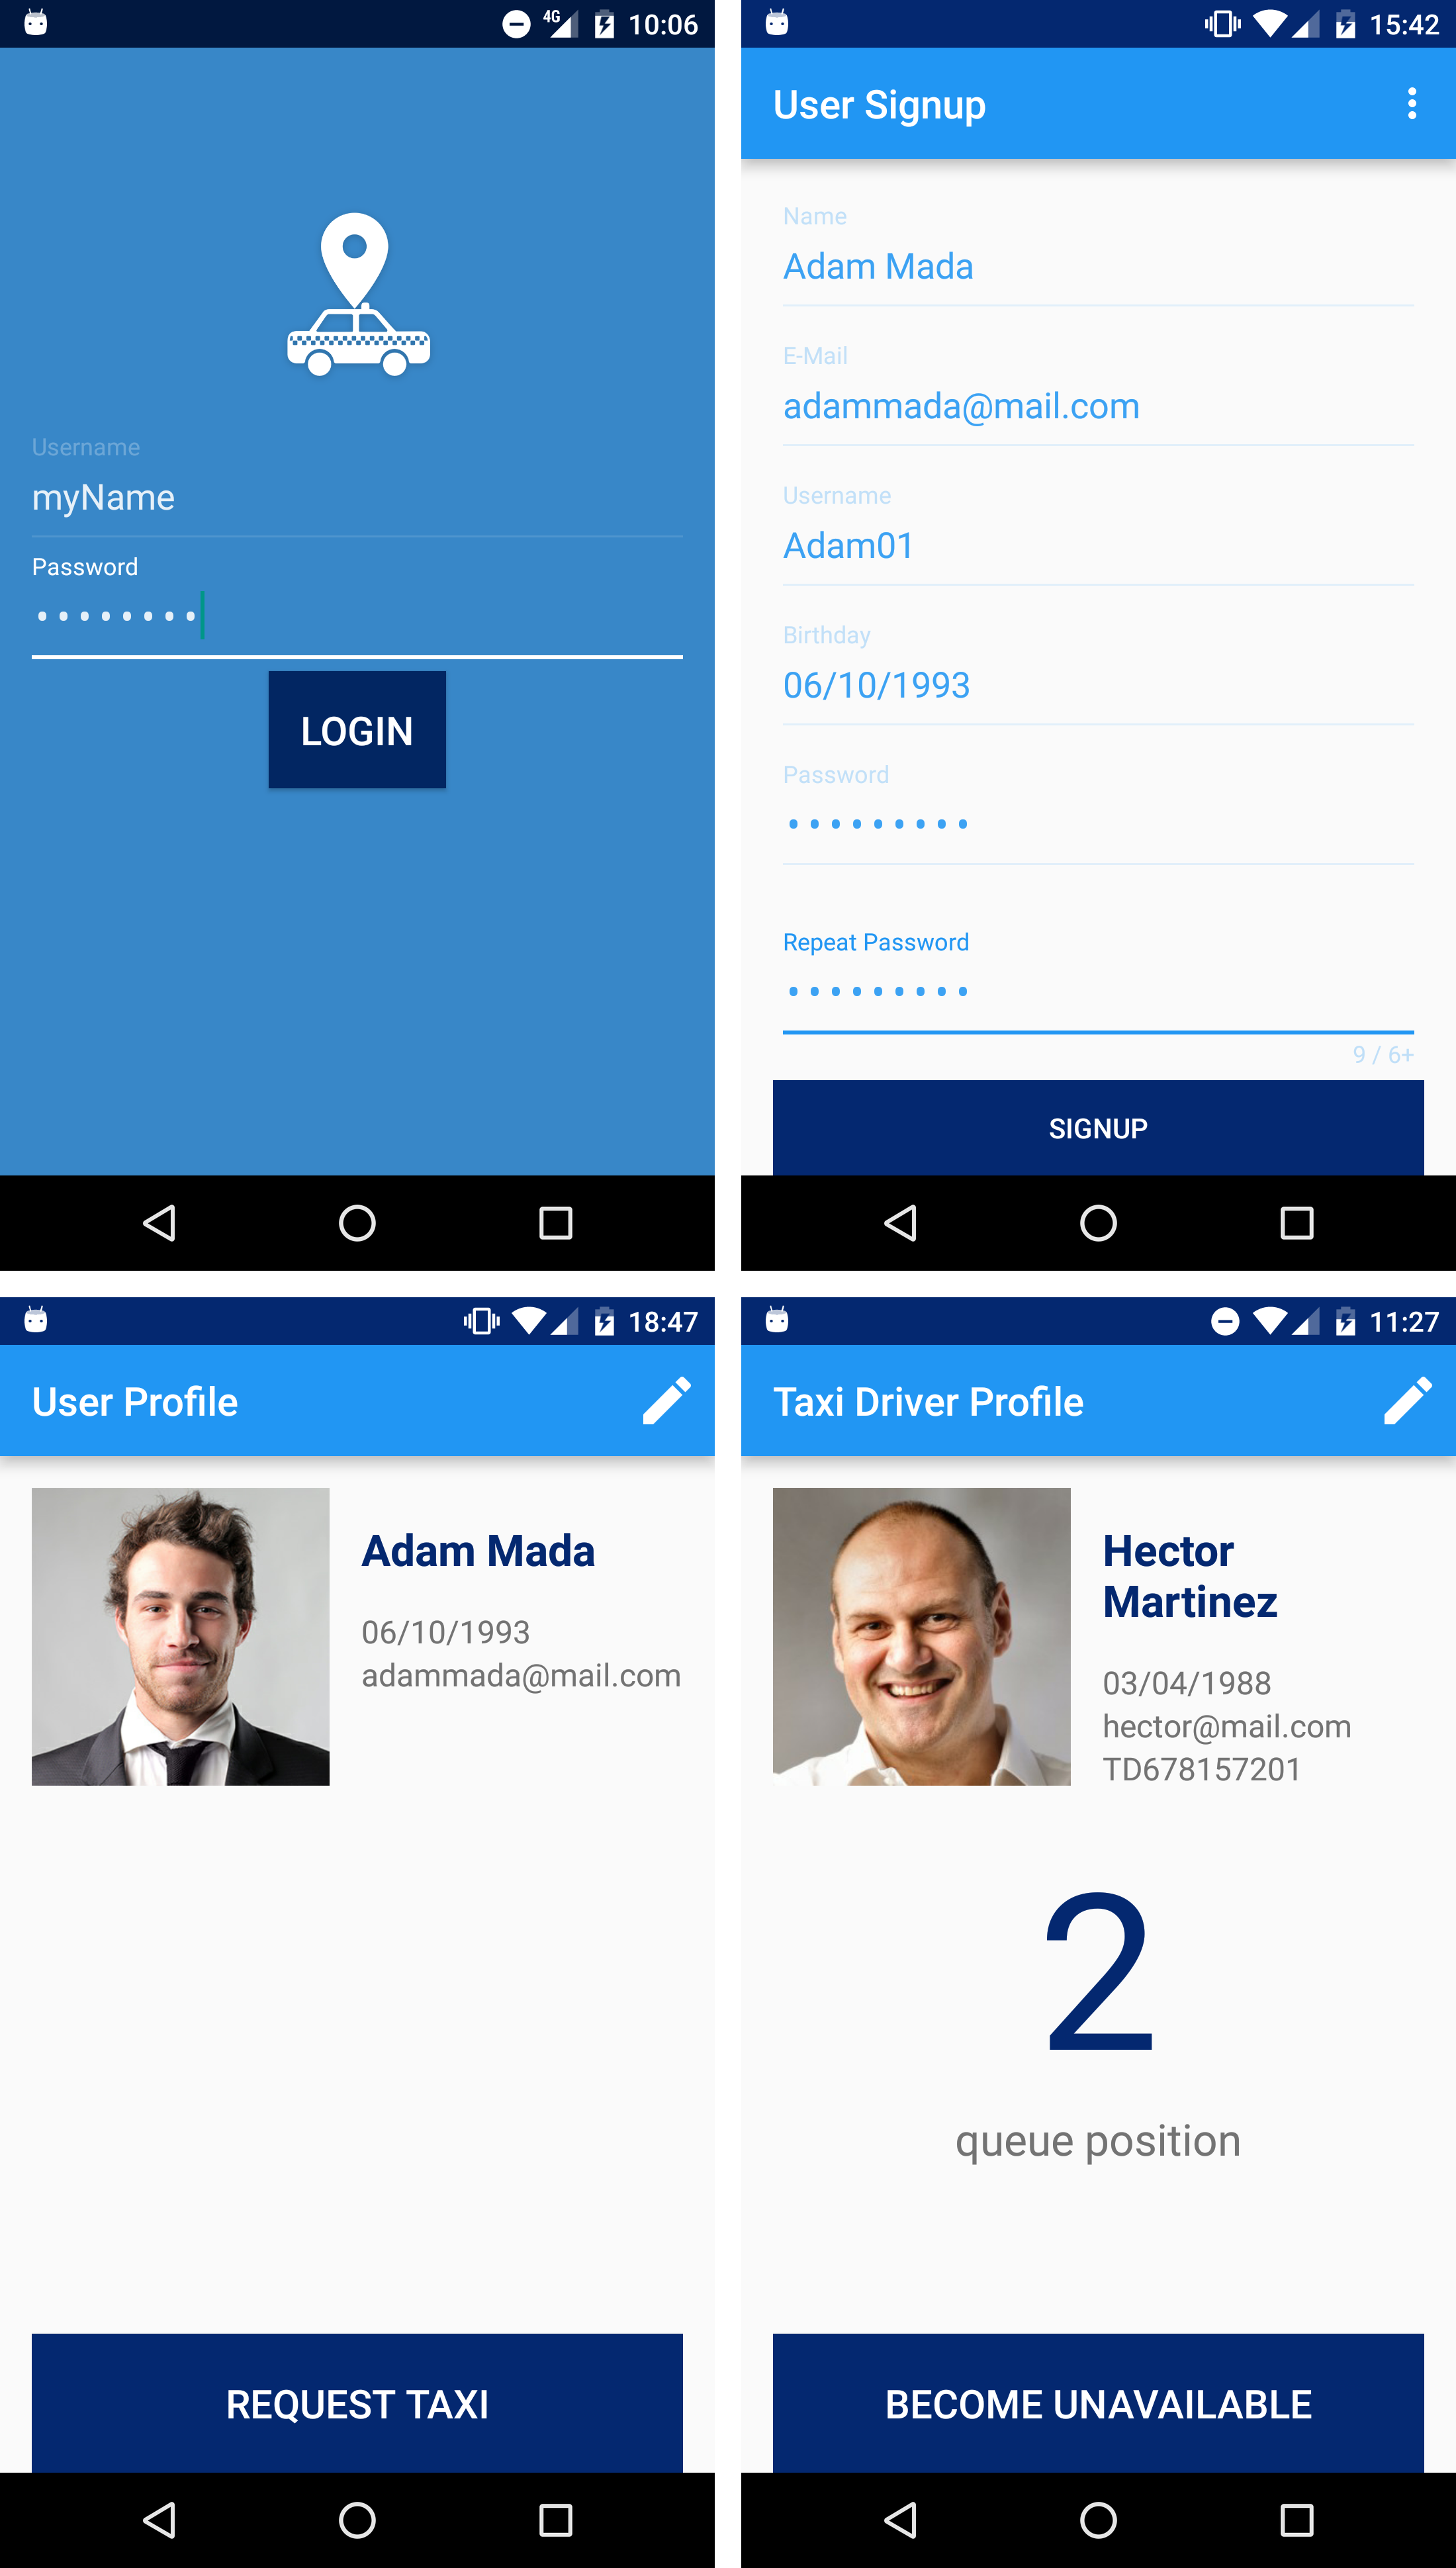
\includegraphics[height=0.9\textheight]{Mockups/mockup1}
\par\end{center}

\begin{center}
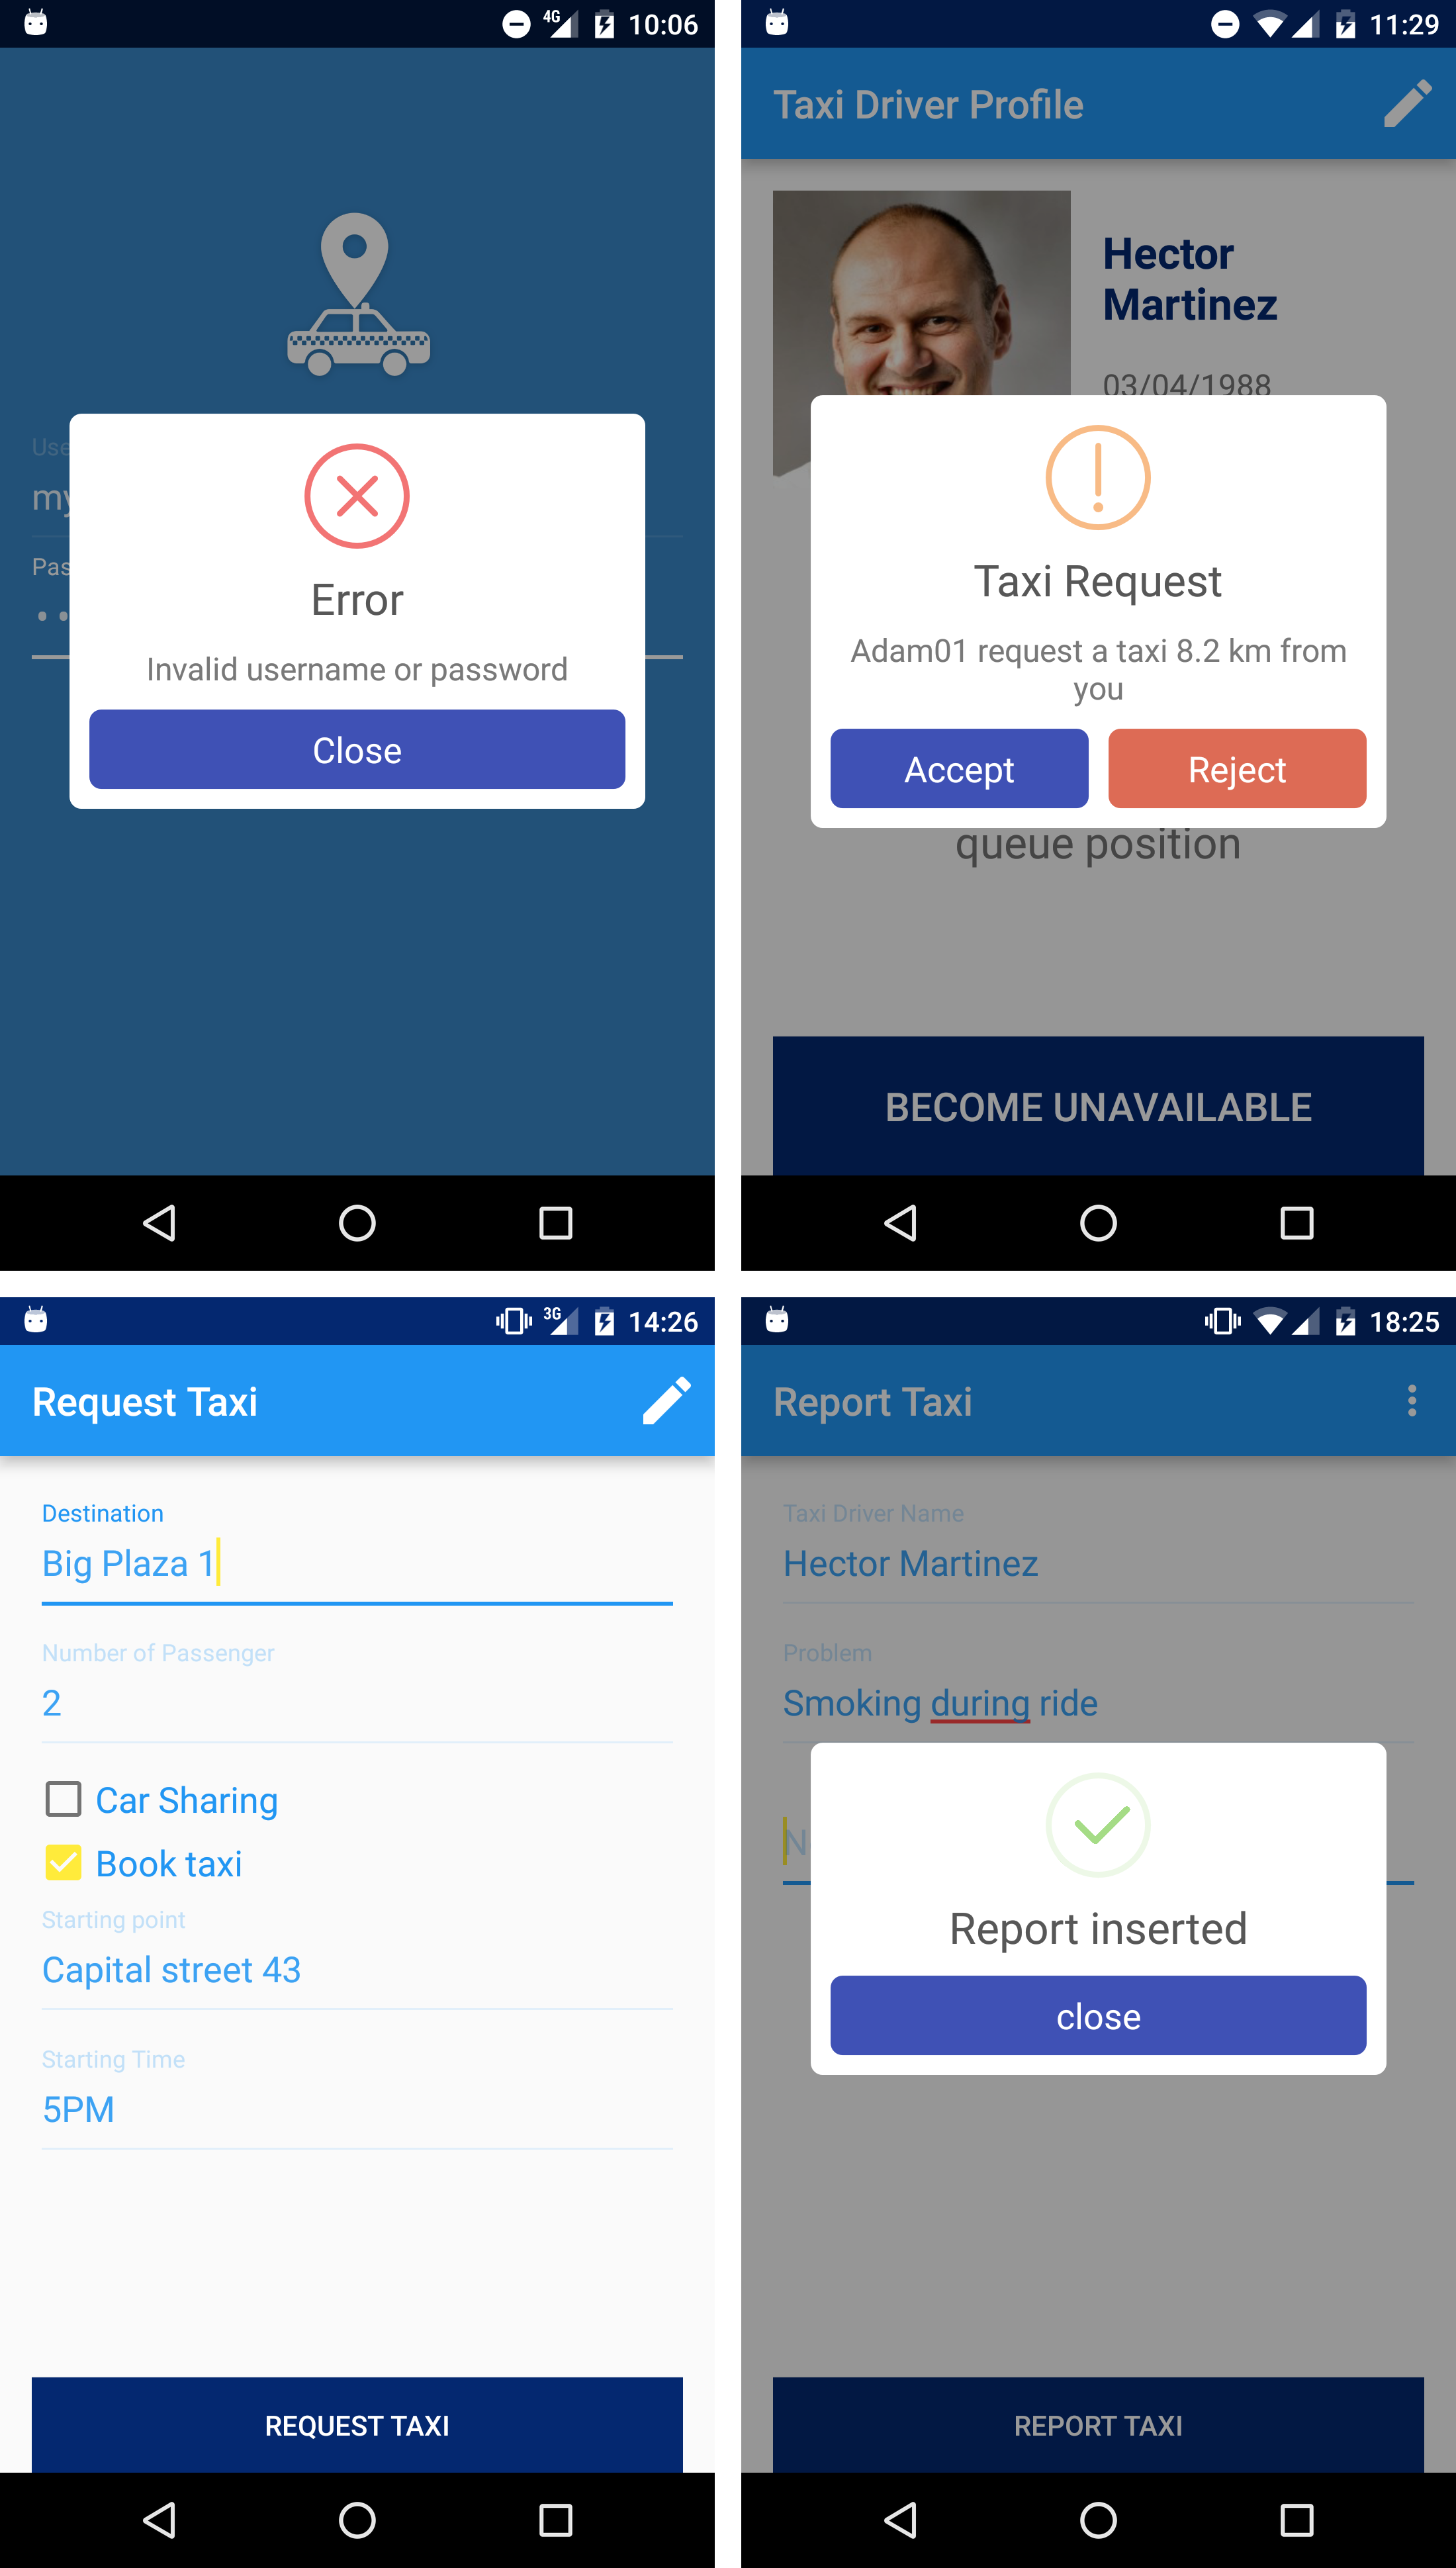
\includegraphics[height=0.9\textheight]{Mockups/mockup2}
\par\end{center}

\begin{center}
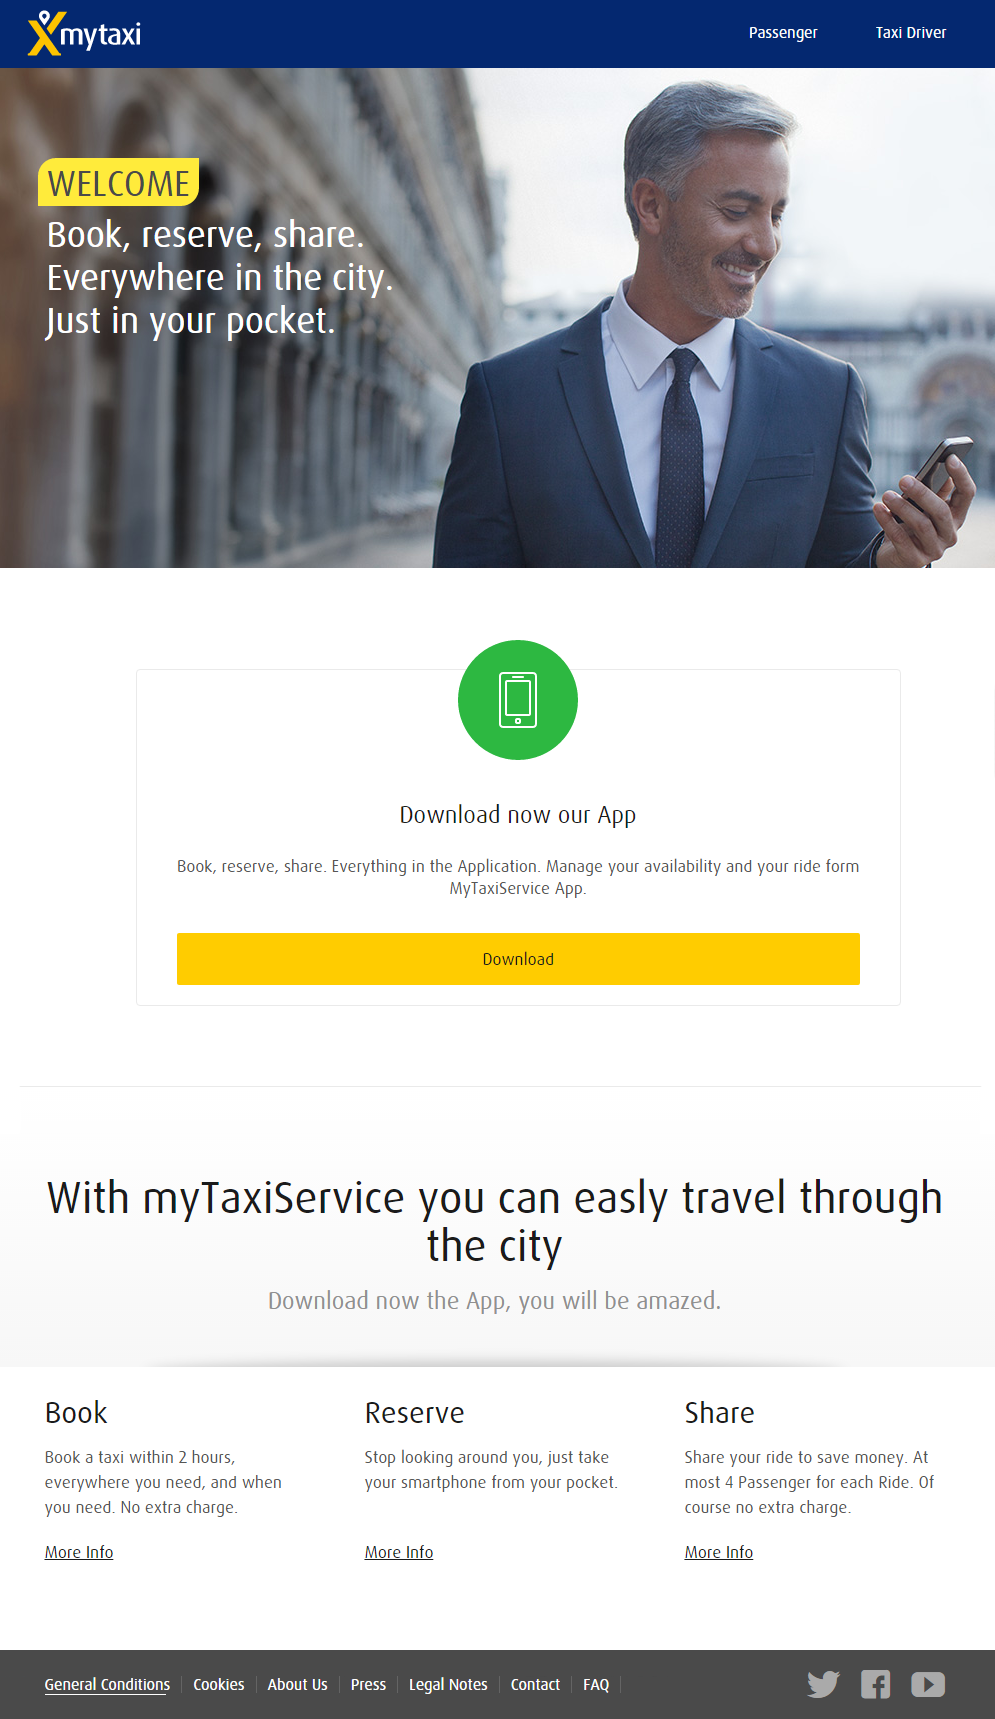
\includegraphics[height=0.9\textheight]{Mockups/Web}
\par\end{center}


\subsection{Functional requirements}

The following set of functional requirements must be kept as official
reference for all further phases of development of the platform.

These requirements are meant as a more in-depth description of the
main system functionalities listed in sec. \ref{sub:Product-functions},
and must be considered alongside the domain assumptions in sec. \ref{sub:Domain-Assumptions}.


\subsubsection{Back-end requirements\label{sub:Back-end-requirements}}
\begin{enumerate}
\item The system must act as the central point of communication between
taxi drivers and customers (functions F1 and F4).

\begin{enumerate}
\item The system must forward the customers' requests to taxi drivers. 
\item The system must forward the taxi drivers' replies (in response to
requests of point 1.(a)) to customers. 
\item The system must manage the exceptions that may happen in the flow
of events (see sec. \ref{sub:Flow-of-events} for more specific description
of these exceptions) 
\end{enumerate}
\item The system must manage the customers taxi reservation requests and
forward them to taxi drivers when necessary. (functions F1 and F4). 
\item The system must manage the taxi queues associated to the different
zones of the city (function F9).

\begin{enumerate}
\item The application must keep track of the availability statuses of all
taxi drivers (also see req. 3, sec. \ref{sub:Taxi-side-application-specific})
and manage the queues accordingly. 
\end{enumerate}
\item The system must manage the operational databases.

\begin{enumerate}
\item The system must store user operation critical data (username, password,
e-mail address, name, date of birth). 
\item The system must keep track of changes in user information when prompted
(functions F2 and F5). 
\item The system must store user records submitted through the \textit{Report}
functions (functions F3 and F6). 
\end{enumerate}
\item The system must perform the necessary validation and consistency checks
on any data it handles in order to ensure the functional and non functional
requirements listed in the following sections. 
\end{enumerate}

\subsubsection{Generic user application requirements}
\begin{enumerate}
\item The application must act as external interface between users and the
back-end.

\begin{enumerate}
\item The application must enable users to register into the platform. 
\item The application must enable users to log into the platform. 
\item The application must provide users with an interface to manage their
personal information (functions F2 and F5). 
\end{enumerate}
\item The application must enable registered users to retrieve a forgotten
password (by sending them a temporary password on the email address
associated to the account)
\item The application must display confirmations and error messages forwarded
by the back-end (see sec. \ref{sub:Flow-of-events} and req. 1, sec.
\ref{sub:Back-end-requirements}). 
\item The application must provide all the implementation-specific requirements
listed in the following sections. 
\end{enumerate}

\subsubsection{Taxi-side application specific requirements\label{sub:Taxi-side-application-specific}}
\begin{enumerate}
\item The application must notify the taxi driver when a request from a
customer is forwarded by the back-end (function F4). 
\item The application must show the taxi driver's position in their queue. 
\item The application must enable the taxi driver to toggle their availability
status between \textit{available }and \textit{unavailable}. 
\item The application must enable the taxi driver to submit \textit{Customer}
reports (function F6).

\begin{enumerate}
\item The application must require information about the ride if the information
is not directly deductible from the known data. 
\end{enumerate}
\item The application must enable the taxi driver to submit \textit{Technical
problem} reports (function F7).

\begin{enumerate}
\item The application must require information about the technical problem
before submitting the report to the system. 
\item The application must require the taxi driver to state whether they
want a replacement to complete the ride (if the technical problem
happens when a passenger is on board) before submitting the report
to the system. 
\end{enumerate}
\end{enumerate}

\subsubsection{Customer-side application specific requirements\label{sub:Customer-side-application-specif}}
\begin{enumerate}
\item The application must enable the customer to request the services of
a taxi. (function F1).

\begin{enumerate}
\item The application must enable the customer to request a taxi in the
very short term (the service is exploited as soon as the taxi is available). 
\item The application must enable the customer to reserve a taxi in advance.

\begin{enumerate}
\item The application must require the customer's destination before submitting
this kind of request to the system. 
\end{enumerate}
\item The application must enable the customer to select the \textit{Taxi
sharing} option (it allows users with similar routes at the same hour
to share the taxi and split the fee)

\begin{enumerate}
\item The application must require the customer's starting point and destination
before submitting this kind of request to the system. 
\end{enumerate}
\item The application must enable the customer to select both options of
points 1.(b) and 1.(c) of this section at the same time. 
\item The application must enable the customer to reserve a ride for more
than 1 person (see req. 4, sec. \ref{sub:Functional-constraints})
\end{enumerate}
\item The application must enable the customer to submit a \textit{Taxi
}reports (function F3).

\begin{enumerate}
\item The application must require information about the ride if the information
is not directly deductible from the known data. 
\end{enumerate}
\end{enumerate}

\subsubsection{Functional constraints\label{sub:Functional-constraints}}
\begin{enumerate}
\item Taxi reservations must can only be issued at least 2 hours before
the requested time of the ride (function F1, associated to req. 1.(b),
sec. \ref{sub:Customer-side-application-specif}). 
\item Requests associated to taxi reservations must be forwarded to taxi
drivers exactly 10 minutes before the requested time (function F9,
associated to req. 1.(b), sec. \ref{sub:Customer-side-application-specif}). 
\item \textit{Taxi} and \textit{Customer }reports must be accepted only
on condition that the ride happened in a 24 hours time frame from
the submission request functions (functions F3 and F6). 
\item A \textit{Ride} object must allow up to 6 possible passenger between
application users (possibly in \textit{Car sharing }mode) and additional
passenger added by a user (see requirement 1.(e), sec. \ref{sub:Customer-side-application-specif})
\end{enumerate}

\subsection{Use cases}

This section contains a graphical UML description of the possible
use cases of the platform, associated to the respective actors.

A more in-depth description of the use cases will be given in secs.
\ref{sub:Scenarios} and \ref{sub:Flow-of-events}.

\begin{center}
\includegraphics[width=1\textwidth]{\string"Use_cases_and_Sequence_diagram/SequenceDiagrams svg/svg/Model1__UseCaseDiagram1_17\string".eps}
\par\end{center}


\subsection{Entities and objects}


\subsubsection{Logical database requirements}

The majority of data processed by the DBMS consists of Java \textit{String
}and \textit{Date }objects. Images and complex objects might be stored
in the database, too, and must therefore be considered during the
design of the database.

The majority of stored data is not frequently accessed as most of
the operational variables are strictly mutable (users' positions,
queues, non-booked rides) and therefore not needed to be stored.

Stored data might consist of stable personal information of the users
and, while not immutable, it can be considered as rarely accessed.

A deeper insight on the data classes and operational variables is
found in the next sections of this document, so it is advised to keep
this section only as a general reference and to approach the design
of the database by looking at the more specific descriptions given
there.


\subsubsection{Class diagram \label{sub:Class-diagram}}

\begin{center}
\includegraphics[width=1\textwidth]{\string"Use_cases_and_Sequence_diagram/SequenceDiagrams svg/svg/Model2__ClassDiagram1_20\string".eps}
\par\end{center}

\pagebreak{}


\subsubsection{Entity behaviors\label{sub:Entity-Behaviors}}
\begin{itemize}
\item[{{{{\textbf{{[}EB1{]}}}}}}] \textbf{Taxi driver}


Taxi drivers, once logged in, can choose to toggle their availability
between the two main statuses \textit{Available }(if the driver is
waiting for incoming requests and is in a local queue) and \textit{Unavailable
}(if the driver is unable or unwilling to accept new requests; this
applies also to drivers who are carrying passengers, who are automatically
considered \textit{unavailable} once the accept a request).

\end{itemize}
\pagebreak{}
\begin{itemize}
\item[{{{{\textbf{{[}EB2{]}}}}}}] \textbf{Ride }
\end{itemize}
\begin{center}
\includegraphics[height=0.9\textheight]{\string"Use_cases_and_Sequence_diagram/SequenceDiagrams svg/svg/StateMachine2__Ride_22\string".eps} 
\par\end{center}

\pagebreak{}
\begin{itemize}
\item[{{{{\textbf{{[}EB3{]}}}}}}] \textbf{Queue manager }


The queue manager is the software component in charge of smartly managing
the local queues and reservations scheduling in the platform. It has
access to all the instances of \textit{ride, taxi driver }and \textit{customer}
objects and can modify these objects' statuses in reaction to different
events. 


The core algorithms of the queue manager have to:
\begin{itemize}
\item Handle one local queue for each zone of the town.
\item Respond to taxi drivers' replies to customer requests.

\begin{itemize}
\item If a taxi driver accepts a ride request, they must be de-queued and
set as \textit{Unavailable}.
\item If a taxi driver refuses a ride request, they must be de-queued and
set as \textit{Unavailable}\footnote{This behavior is different from the initial customer specification;
it has been modified to prevent a possible unwanted situation in which
all the taxi drivers in a queue refuse the request and:
\begin{enumerate}
\item The taxi drivers are continuously notified with the customer's request.
\item The user never gets a failure notification, because the system is
kept looping through a \textit{de-facto} unavailable queue. \end{enumerate}
}. 
\item If a taxi driver notifies a technical problem (function F7 of sec.
\ref{sub:Product-functions}), they must be de-queued and set as \textit{Unavailable. }
\end{itemize}
\item Keep track of all the customer ride reservations and manage eventual
changes.

\begin{itemize}
\item Dynamically assign taxi drivers to a customer when the requested time
arrives.
\item Respond to changes in a customer's reservation (consistency checks
are carried out by other components of the platform) and possibly
remove the request from the schedule. 
\end{itemize}
\end{itemize}
\end{itemize}

\subsection{Scenarios\label{sub:Scenarios}}

To help the reader understand the above stated requirements, a brief
description of how a use case might look like in the real world is
given below.

In the examples, Adam, Michelle and Joanne are customers who intend
to request a taxi and Hector, Monica, Jim and Samuel are taxi drivers
of the town.


\subsubsection{Sign up}

Adam has just downloaded the customer-side app and wants to sign up
into the platform. He requests the customer registration page, fills
the form and submits the request to the system. If Adam's e-mail and
username are unique, the system gives Adam a confirmation of the success
of the operation and redirects Adam to the login page; otherwise,
an error message is displayed on Adam's phone.


\subsubsection{Login}

Adam, now registered, inserts the username and password in the login
form and clicks the login button; the system checks the information
and, if the username-password combination is correct, redirects Adam
to his own user profile page; otherwise, an error message is displayed
on Adam's phone.


\subsubsection{Available}

Hector, already logged into the platform, starts his working by day
opening his taxi-side application and communicating his availability
to the system. The system updates the taxi queue in Hector's zone
and sends Hector a notification with his position in the queue.


\subsubsection{Taxi request\label{sub:Taxi-request}}

Adam, now logged into the system, wants to book a taxi to go home.
He opens the taxi request page on the app, and requests a taxi. The
system forwards Adam's request to the queue associated with Adam's
position (tracked by the GPS on Adam's phone), and Hector, which is
the first taxi driver in the queue, is notified with the request.

Unfortunately, Hector has now decided to take a break and does not
want to take charge of this ride; he refuses Adam's request by tapping
a button on the app, and the system forwards the request to Monica,
the taxi driver immediately after Hector in the queue.

As she accepts Adam's request, Adam receives a notification on the
app with the estimated waiting time.


\subsubsection{Book a taxi\label{sub:Book-a-Taxi}}

While on Monica's taxi, Adam wants to book a taxi for that evening
at 6 PM, in order to go to the cinema. He opens the \textit{Taxi request}
page of the app, and fills and submits the request form.

The system checks the information (sending eventual error notifications
back to Adam) and creates a \textit{Ride }object which will be kept
in a \textit{Pending} status.

Ten minutes before 6PM the system will forward Adam's request to the
first taxi in the queue at that time, and similarly to the previous
scenario a taxi will be assigned to Adam.


\subsubsection{Car sharing}

Michelle and Joanne live in the same neighborhood, and they both decide
to go see a fair on the other side of the Town. Since they are both
short on money, after opening the \textit{Taxi request }page of the
app they both check the \textit{car sharing }option; after checking
the option, the apps automatically adds a field in the reservation
form in which they must specify their intended destination; they then
submit their requests.

The system performs a check on Michelle and Joanne's requests and,
since their routes match, it automatically assign them to the same
taxi.

Based on whether they decided to book the taxi or simply request it,
the taxi will be chosen similarly to scenarios \ref{sub:Book-a-Taxi}
or \ref{sub:Taxi-request} respectively.


\subsubsection{Manage \textit{Reserve taxi} request}

Later that day, Adam browses the platform's website from his laptop's
browser, and opens the \textit{Manage taxi request} page to change
the booking time from 6PM to 7PM.

The system checks whether Adam's request is acceptable (there must
be at least two hours between the current time and the requested time),
and possibly modifies to time on which to forward the request to the
queue.


\subsubsection{Report taxi}

Jim picks Adam up at 7PM. During the ride Jim lights up a cigarette
and is unreasonably rude towards Adam.

Adam opens the \textit{Report taxi} page on the app, to file a complaint
about Jim's behavior. The system updates Jim's record with the new
report and confirms the success of the operation to Adam.


\subsubsection{Report customer}

After the ride, Adam is annoyed by the behavior of Jim and refuses
to pay for the ride.

Jim opens the \textit{Report user} page, fills the complaint form
and submits it to the system. The system updates Adam's record with
the new report and confirms the success of the operation to Jim.


\subsubsection{Manage personal information}

Joanne has opened a new main email account.

She opens her profile page from the app, clicks on the \textit{edit}
button and changes her email address to match the new one; she then
submits the new information.

The system performs a check on the information, updates Joanne's profile
and notifies the success of the operation to Joanne.


\subsubsection{Report problem}

During a ride, Hector has a problem with his taxi's engine and can't
bring Joanne to her destination.

Through the \textit{Report problem} page of the app, he notifies the
problem to the system by filling the form and submitting. The system
acknowledges the report and asks Hector if he'll be needing a new
taxi; Hector confirms, and the system forwards his request to Samuel,
who is the first taxi driver in Hector and Joanne's current zone.


\subsection{Flow of events\label{sub:Flow-of-events}}

This section contains a description of how different use cases should
happen, divided in sequential steps. The participating actor are those
described in sec. \ref{sub:Actors-and-related}.


\subsubsection{Sign-up}

\begin{center}
\begin{tabular}{lp{8cm}}
\hline 
Actors  & A1 - Guest\tabularnewline
\hline 
Preconditions  & The guest is not registered into the system.\tabularnewline
\hline 
Execution Flow  & \begin{enumerate}
\item The guest requests the registration page. 
\item The guest fills the registration form and submits the request. 
\item The system checks the uniqueness of the username and e-mail. 
\item The system creates the customer (or taxi driver) profile . 
\item The system sends the confirmation to the guest.\end{enumerate}
\tabularnewline
\hline 
postconditions  & The guest is now a registered user.\tabularnewline
\hline 
Exceptions  & The e-mail or username are not unique or, in the case of a taxi driver
sign-up, the license is not valid: an error message is shown. \tabularnewline
\end{tabular}
\par\end{center}

\begin{center}
\includegraphics[width=1\textwidth]{\string"Use_cases_and_Sequence_diagram/SequenceDiagrams svg/svg/Collaboration1__Interaction1__Signup_2\string".eps}
\par\end{center}


\subsubsection{Login}

\begin{center}
\begin{tabular}{lp{8cm}}
\hline 
Actors  & A1 - Guest \tabularnewline
\hline 
Preconditions  & The guest is already registered into the system.\tabularnewline
\hline 
Execution Flow  & \begin{enumerate}
\item The guest requests the login page. 
\item The guest fills the form and submits the request. 
\item The system checks the username and password. 
\item The system sends a login confirmation. 
\item The guest is logged into the system. 
\item The guest is redirected to the user main page.\end{enumerate}
\tabularnewline
\hline 
postconditions  & The guest is now a logged-in user.\tabularnewline
\hline 
Exceptions  & The username-password combination is incorrect, so the guest cannot
log in: an error message is shown.\tabularnewline
\end{tabular}
\par\end{center}

\begin{center}
\includegraphics[height=1\textheight]{\string"Use_cases_and_Sequence_diagram/SequenceDiagrams svg/svg/Collaboration2__Interaction1__Login_3\string".eps}
\par\end{center}


\subsubsection{Available}

\begin{center}
\begin{tabular}{lp{8cm}}
\hline 
Actors  & A3 - Taxi driver \tabularnewline
\hline 
Preconditions  & The taxi driver is logged into the system.\tabularnewline
\hline 
Execution Flow  & \begin{enumerate}
\item The taxi driver opens the app. 
\item The taxi driver changes their availability by tapping a button: a
request is sent to the system. 
\item The system updates the queue. 
\item The system returns a confirmation to the taxi driver. \end{enumerate}
\tabularnewline
\hline 
postconditions  & The taxi driver has now changed their availability.\tabularnewline
\hline 
Exceptions  & \begin{itemize}
\item The taxi driver is located in a invalid zone and they try to become
\textit{available}: an error message is shown. \end{itemize}
\tabularnewline
\end{tabular}
\par\end{center}

\begin{center}
\includegraphics[width=1\textwidth]{\string"Use_cases_and_Sequence_diagram/SequenceDiagrams svg/svg/Collaboration10__Interaction1__Available_11\string".eps}
\par\end{center}


\subsubsection{Taxi request}

\begin{center}
\begin{longtable}{l>{\raggedright}p{8cm}}
\hline 
Actors  & A2.1 - Customer, A3 - Taxi driver \tabularnewline
\hline 
Preconditions  & Both users must be logged in, the taxi driver must be available.\tabularnewline
\hline 
Execution Flow  & \begin{enumerate}
\item The customer requests the \textit{Taxi request} page 
\item The customer fills the request form according to their preference
and sends the information to the system: they can choose to request
a ride for a certain number of passengers, reserve a taxi or enable
the \textit{Taxi sharing }option. 
\item Based on the type of request that the customer issued, the system
generates a request with all the needed data and commits it to the
\textit{Queue manager }(entity E3, sec. \ref{sub:Entity-Behaviors})
\item The taxi driver can either ignore the request or accept it. 
\item If the taxi driver accepts the request, the system notifies to the
customer the incoming taxi (with an approximate ETA) and changes the
availability of the taxi driver; otherwise, the system puts the taxi
driver at the end of the queue and forwards the request to the next
first taxi driver of the queue. 
\item If the issued request was a booking request or a request with \textit{Taxi
sharing }enabled, the system calculates the estimated fee for the
passenger and adds it to the notification sent to the user. \end{enumerate}
\tabularnewline
\newpage
\hline 
postconditions  & If the request is accepted by a taxi driver, the customer is now a
passenger.\tabularnewline
\hline 
Exceptions  & \begin{itemize}
\item The customer provides incorrect information in the request form: an
error notification is shown. 
\item No taxis are available: the system notifies so to the user. 
\item The customer is not in a valid position (\emph{e.g. outside the town}):
an error notification is shown. \end{itemize}
\tabularnewline
\end{longtable}
\par\end{center}

\begin{center}
\includegraphics[width=1\textwidth]{\string"Use_cases_and_Sequence_diagram/SequenceDiagrams svg/svg/Collaboration3__Interaction1__Taxi Request_4\string".eps}
\par\end{center}


\subsubsection{Manage \textit{Reserve taxi} request}

\begin{center}
\begin{tabular}{lp{8cm}}
\hline 
Actors  & A2.1 - Customer\tabularnewline
\hline 
Preconditions  & \begin{itemize}
\item The customer must have reserved a taxi. 
\item The customer must be logged in.\end{itemize}
\tabularnewline
\hline 
Execution Flow  & \begin{enumerate}
\item The customer requests the \textit{Taxi request management} page. 
\item The customer can modify the request by filling a\textit{ }form and
submitting it, or delete the request by tapping (or clicking) a button. 
\item The system modifies the request and returns a confirmation to the
passenger. 
\item The request is forwarded to the right local queue accordingly; if
the user canceled their request, the request is not sent. \end{enumerate}
\tabularnewline
\hline 
postconditions  & \begin{itemize}
\item If the customer chooses to modify the request, the request is updated. 
\item If the customer chooses to delete the request, the request is canceled.\end{itemize}
\tabularnewline
\hline 
Exceptions  & \begin{itemize}
\item The customer provides incorrect information in the \textit{Modify
request} form: an error message is shown. 
\item The customer tried to cancel their request too late: an error message
is shown and the modification is not allowed.\end{itemize}
\tabularnewline
\end{tabular}
\par\end{center}

\begin{center}
\includegraphics[width=1\textwidth]{\string"Use_cases_and_Sequence_diagram/SequenceDiagrams svg/svg/Collaboration15__Interaction1__Manage Taxi Request_19\string".eps}
\par\end{center}


\subsubsection{Report taxi}

\begin{center}
\begin{tabular}{lp{8cm}}
\hline 
Actors  & A2.2 - Passenger \tabularnewline
\hline 
Preconditions  & \begin{itemize}
\item The interaction between the passenger and the taxi driver must have
happened at most 24 hours before. 
\item The passenger must be logged in.\end{itemize}
\tabularnewline
\hline 
Execution Flow  & \begin{enumerate}
\item The passenger requests the \textit{Report taxi} page. 
\item The passenger fills the form and submits the report. 
\item The system checks the submitted data. 
\item The system updates the taxi driver's record. 
\item The system notifies to the passenger the success of the operation.\end{enumerate}
\tabularnewline
\hline 
postconditions  & The taxi driver is reported by the passenger.\tabularnewline
\hline 
Exceptions  & The passenger provides incorrect information in the report form: an
error message is shown. \tabularnewline
\end{tabular}
\par\end{center}

\begin{center}
\includegraphics[width=1\textwidth]{\string"Use_cases_and_Sequence_diagram/SequenceDiagrams svg/svg/Collaboration7__Interaction1__Report Taxi_8\string".eps}
\par\end{center}


\subsubsection{Report customer}

\begin{center}
\begin{tabular}{lp{8cm}}
\hline 
Actors  & A3 - Taxi driver \tabularnewline
\hline 
Preconditions  & \begin{itemize}
\item The interaction between the passenger and the taxi driver must have
happened at most 24 hours before. 
\item The taxi driver must be logged in.\end{itemize}
\tabularnewline
\hline 
Execution Flow  & \begin{enumerate}
\item The taxi driver requests the \textit{Report customer} page. 
\item The taxi driver fills the form and submits the report. 
\item The system checks the submitted data. 
\item The system updates the customer's record. 
\item The system notifies to the taxi driver the success of the operation.\end{enumerate}
\tabularnewline
\hline 
postconditions  & The customer is reported by the taxi driver.\tabularnewline
\hline 
Exceptions  & The taxi driver provides incorrect information in the report form:
an error message is shown. \tabularnewline
\end{tabular}
\par\end{center}

\begin{center}
\includegraphics[width=1\textwidth]{\string"Use_cases_and_Sequence_diagram/SequenceDiagrams svg/svg/Collaboration13__Interaction1__Report Customer_14\string".eps}
\par\end{center}


\subsubsection{Manage personal information}

\begin{center}
\begin{tabular}{lp{8cm}}
\hline 
Actors  & A2 - Customer or A3 - Taxi driver \tabularnewline
\hline 
Preconditions  & The user must be logged in.\tabularnewline
\hline 
Execution Flow  & \begin{enumerate}
\item The user requests their profile page. 
\item The user's personal information is shown on the user's application. 
\item The user can begin editing their profile information by tapping (or
clicking) on the \textit{Edit} button. 
\item The user edits their information and submits the changes to the system. 
\item The system performs a check on the new information. 
\item If the information is correct, a confirmation is sent back to the
user.\end{enumerate}
\tabularnewline
\hline 
postconditions  & The user profile information is changed.\tabularnewline
\hline 
Exceptions  & The user provides incorrect information: an error message is shown. \tabularnewline
\end{tabular}
\par\end{center}

\begin{center}
\includegraphics[width=1\textwidth]{\string"Use_cases_and_Sequence_diagram/SequenceDiagrams svg/svg/Collaboration9__Interaction1__Manage your Personal Info_10\string".eps}
\par\end{center}


\subsubsection{Report problem}

\begin{center}
\begin{tabular}{lp{8cm}}
\hline 
Actors  & A3 - Taxi driver \tabularnewline
\hline 
Preconditions  & The taxi driver must be logged in\tabularnewline
\hline 
Execution Flow  & \begin{enumerate}
\item The taxi driver requests the \textit{Report problem} page. 
\item The taxi driver fills the form and submits the information regarding
a technical problem that they are experiencing. 
\item If the taxi driver has a passenger on board, they can request another
taxi to drive the passenger to their destination. 
\item If the taxi driver requests another taxi the system looks for an available
taxi driver, with the usual procedure. 
\item If a taxi driver accepts the request, a confirmation is sent to the
driver who is submitting the report.\end{enumerate}
\tabularnewline
\hline 
postconditions  & The technical problem is reported to the system \tabularnewline
\hline 
Exceptions  & \begin{itemize}
\item The taxi driver is located in a invalid zone: an error message is
shown. 
\item The taxi driver requests a second taxi, but no available taxi is found:
an error message is shown to the user. \end{itemize}
\tabularnewline
\end{tabular}
\par\end{center}

\begin{center}
\includegraphics[width=1\textwidth]{\string"Use_cases_and_Sequence_diagram/SequenceDiagrams svg/svg/Collaboration14__Interaction1__Notify Problem_18\string".eps}
\par\end{center}

\pagebreak{}


\subsection{Performance requirements}

Some non functional requirements regarding performance have been identified
as follows.


\subsubsection{Back-end performance}
\begin{enumerate}
\item The platform must support a number users equals to 3 times the number
of registered taxi drivers in the Town. Estimates must be calculated
each year and modifications to the infrastructure must be made accordingly. 
\item The system must process 99\% of requests in less than 5 seconds. 
\item The system must support parallel processing of the request to a degree
proportional to at least 25\% of the average number of requests. 
\item Management of the database must be transparent to the user, which
must have the impression of a continuous interaction with the system. 
\item Estimates of the costs of the rides must be precise with a 10\% error
margin. 
\item Estimates of the taxi drivers' ETA must be precise with a 10\% error
margin. 
\end{enumerate}

\subsubsection{User-side performance}
\begin{enumerate}
\item The mobile user-side applications must be as energy efficient as possible,
in order to not drain the battery on the users' mobile devices. 
\item The users' profile pictures must have a resolution smaller than 1000x1000
pixels, in order to be efficiently stored, loaded into RAM, and transmitted. 
\end{enumerate}

\subsection{Availability and reliability requirements}

Since MyTaxiService is a service-oriented platform, its reliability
parameters directly relate to its availability parameters. The platform's
ability to function under the stated conditions is indeed its ability
to respond to users' requests at any given time, hence the strict
relation between the two. It has been decided to treat the two aspect
as one, and the related non functional requirements are listed in
this section. 
\begin{enumerate}
\item The platform's services must be available to the users 24/7. 
\item The RTO parameter must be kept at minimal levels (less than 1 minute)
at any given time.

\begin{enumerate}
\item Mission critical data must be locally mirrored on fast hardware (e.g.
stored in RAID1 arrays with flash storage). 
\end{enumerate}
\item The RPO parameter must be kept at minimal levels (less than 10 seconds)
at any given time.

\begin{enumerate}
\item Any data must be locally stored in a 10 second time frame from its
creation. 
\item Any locally stored data must be locally and remotely mirrored in a
1 minute time frame from its memorization. 
\end{enumerate}
\item Data integrity checks must be periodically performed between the main
data storage unit and the secondary backups, in order to ensure the
success of disaster recovery operations. 
\item The implementation of the platform must prefer the absence of service
to an incorrect or unsound one.

\begin{enumerate}
\item No data exchanges must happen during the disaster recovery operations. 
\item Data stored in memory in the event of a system failure or security
breach must be considered corrupt and no attempts must be made at
recovering it. 
\end{enumerate}
\end{enumerate}

\subsection{Security requirements\label{sub:Security-requirements}}

The following non functional requirements cover the security aspects
of the platform in order, among other reasons, to satisfy the constraint
C3, sec. \ref{sub:Constraints}. 
\begin{enumerate}
\item Access to the user data through the intended applications must be
password protected.

\begin{enumerate}
\item A ban system must exists to prevent brute-forcing of the users' passwords. 
\end{enumerate}
\item Sensitive user data (like passwords) must be stored under at least
one encryption layer, after having been \textit{salted}. This applies
to secondary storage, too.

\begin{enumerate}
\item Decryption of the above mentioned data must happen exclusively at
runtime and the \textit{cleartext }information must never be sent
through any communication channels. 
\end{enumerate}
\item Operations on the platform must be performed exclusively by logged
users (with the exception of the guest registration). 
\item HTTP data exchanges between the back-end and the user-side applications
must be encrypted with a recognized SSL certificate (HTTPS protocol). 
\item Access to the back-end system must be protected both via hardware
and software means.

\begin{enumerate}
\item A physical firewall must exists between the Internet and the back-end
main router. 
\item Access to the system must be enabled via IP address whitelisting,
rather than blacklisting. 
\item Root login must be disabled for remote sessions. 
\item Password login must be disabled and signed PKA must be enforced, for
any type of session. 
\item Access logs must be kept, backed up, and regularly analyzed. 
\end{enumerate}
\item Mission critical data must be stored with particular attention to
data integrity. 
\end{enumerate}

\subsection{Maintainability requirements}

The following non functional requirements regarding the maintainability
of the codebase are meant as a small guideline for programmers and
designers in the development phase. 
\begin{enumerate}
\item The codebase for all developed software must be highly modular to
facilitate possible changes in the platform's functions and possible
integration with other systems; this applies especially to the back-end
modules. 
\item The codebase for all developed software must be thoroughly documented
with both in-code comments and official documentation, in order to
facilitate a possible outsourcing of the maintenance phase. 
\end{enumerate}

\subsection{Portability requirements}

The following non functional requirements consider technical details
of the platform's implementation in order to analyze its portability
requirements.

When seen as a whole, the platform consists mainly of its user-side
applications, and the back-end accounts for about 25\% of the codebase;
nonetheless, since the user-side applications are strictly OS dependent,
as specified in sec. \ref{sub:User-interface}, portability is an
issue which has to be tackled in back-end development, in order to
keep costs to a minimum in the case of possible changes in the platform
(e.g. an integration with a preexisting system). Therefore: 
\begin{enumerate}
\item The back-end software must be developed in Java Enterprise Edition. 
\item Integration with support modules in the back-end must happen through
JEE libraries. 
\item Any system related calls, communication protocols and thread related
calls in the back-end must be OS independent (the use of wrapper libraries
is encouraged over a case-by-case analysis). 
\end{enumerate}

\section{Alloy Modeling}


\subsection{Alloy source code\label{sub:Alloy-source-code}}

\begin{lstlisting}[basicstyle={\normalsize\ttfamily},breaklines=true,keywordstyle={\color[RGB]{242,134,10}},morekeywords={assert, pred, all, no, lone, one, some, check, run, but, let, implies, not, iff, in, and, or, set, sig, Int, int, if, then, else, exactly, disj, fact, fun, module, abstract, extends, open, none, univ, iden, seq},morecomment={[l]{//}},morecomment={[s]{/*}{*/}},commentstyle={\color[RGB]{10,200,10}}]
/**Signatures**/
//Sig for Users, having username and mail
abstract sig User{
	username : MString,
	mail : MString
}{
	username != mail
}

//Sig to identify Customers
abstract sig Customer extends User{}

//Passenger is a Customer how request a taxi
sig Passenger extends Customer{}

//Taxi Driver can be Available
sig TaxiDriver extends User{
	license : MString,
	available : Boolean
}

//Ride has: one TaxiDriver, one Starting position, a set of Passenger and some destination positions
sig Ride{
	start : one Position,
	destinations : some Position,
	transport : set Passenger,
	hasDriver : lone TaxiDriver,
	pending : Boolean
}{
	#transport >= 1 and #transport <= 4 and
	all d:destinations | different[d, start] = True and
	#hasDriver = 1 iff pending = True 
}

//Queue for each city Zone
sig Queue{
	contains : set TaxiDriver
}

//Manager of Queues
one sig QueueManager{
	manage : some Queue
}

/**Support Signatures**/
sig MString{}
sig Float{}

sig Position{
	x : Float,
	y : Float
}

abstract sig Boolean{}
one sig True extends Boolean {}
one sig False extends Boolean {}

/**Facts**/
//All the Passengers are Customers (and also Users)
fact {
	Passenger in Customer
}

//Users are composed by all the TaxiDrivers and Customers
fact {
	User = TaxiDriver + Customer
}

//No repeteaded Positions
fact uniquePositions{
	all p,q:Position | p!=q implies different[p,q] = True 
}

//All the Positions are used in the Ride sig
fact noUselessPositions{
	Ride.start + Ride.destinations = Position
}

//No useless Float sig
fact onlyUsedFloat{
	Position.x + Position.y = Float
}

//A User has unique username and mail
fact uniqueUsers{
	all u,w : User | (u.username = w.username or u.mail = w.mail) iff u=w
}

//A TaxiDriver is identified by his own license
fact uniqueLicense{
	all t1,t2 : TaxiDriver | t1.license = t2.license iff t1 = t2
}

//There are no username equals to mail
fact{
	User.username & User.mail = none
}

//Not exists license equals to username and mail
fact{
	(User.username + User.mail) & TaxiDriver.license = none
 }

//The String used are used only for username, mail and license
fact{
	User.username + User.mail + TaxiDriver.license = MString
}

//a User can be transported at most by one pending Ride
fact{
	all u:Ride.transport | (lone r:Ride | r.pending = True and u in r.transport)
}

//If a Taxi Driver is in a Queue implies his availability
fact taxiInQueueIsAvailable{
	all t:TaxiDriver | t in Queue.contains implies t.available = True else t.available = False
}

//Every Taxi Driver belogns at most to one Queue
fact taxiContainedInOneQueue{
	all q,p:Queue | q!=p implies (all t:q.contains | !t in p.contains)
}

//Every Queue belongs to the QueueManager
fact exacltyOneManager{
	all q:Queue | (one m:QueueManager | q in m.manage)
}

//For each Ride the number of destinations belongs to the # of Passenger
fact maxDestinations{
	all r:Ride | #r.destinations <= #r.transport
}

/**Functions **/
//True if the Positions are different, False otherwise
fun different[p1,p2 : Position] : Boolean{
	(p1.x != p2.x or p1.y != p2.y) implies True else False
}

/**Assertions**/
assert differentsUsernames{
	no u1,u2:User | u1.username = u2.username and u1 != u2
}

assert differentsMail{
	no u1,u2:User | u1.mail = u2.mail and u1 != u2
}

/**Predicates**/
pred taxiDriverAvailable{
	all t:TaxiDriver | t.available = True implies (one q:Queue | t in q.contains)
}

pred intrestingPred{
	#Passenger > 1
	#Position < 3
	#Queue = 2
	#Ride > 0 and #Ride < 3
	#TaxiDriver > 1
	one t:TaxiDriver | t.available = True
	one r:Ride | r.pending = True
}

pred show{}

/**Executions**/
run taxiDriverAvailable for 5
\end{lstlisting}



\subsection{Alloy output}

The output is shown to give a visual confirmation of the consistency
of the model, even if it does not add any further information to the
document.

Note that passengers and taxi drivers can be related to more than
one ride; this is done intentionally, as ride objects do not cease
to exist once the ride is completed, but are stored and are associated
with the user's history.

\begin{center}
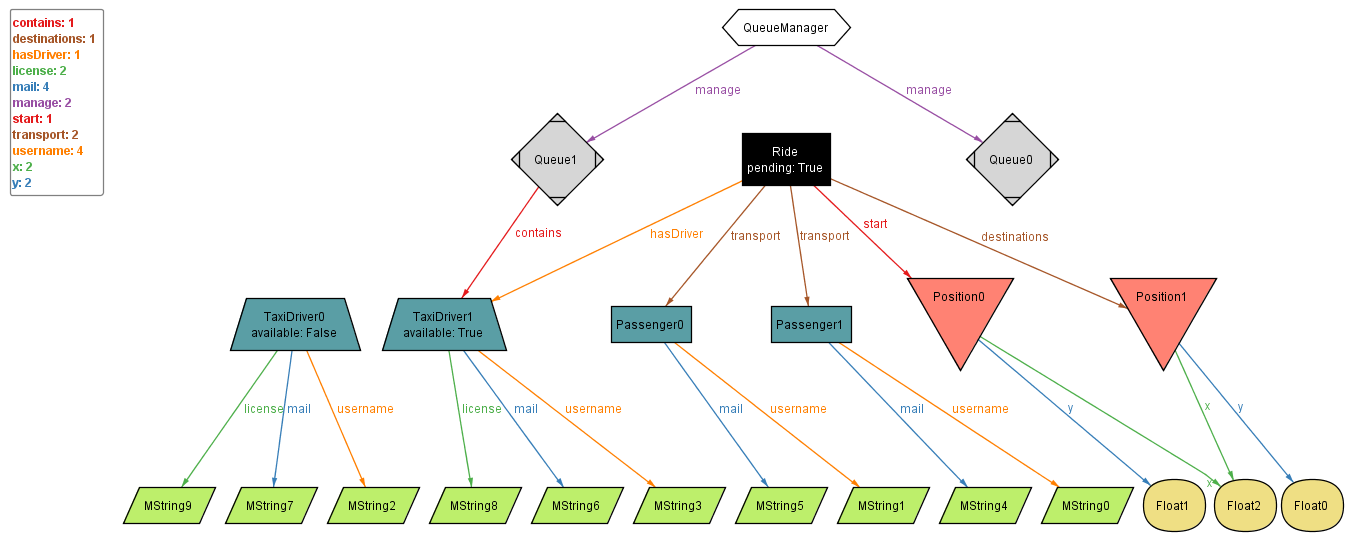
\includegraphics[angle=90,height=0.9\textheight]{instance} 
\par\end{center}

\pagebreak{}

\begin{center}
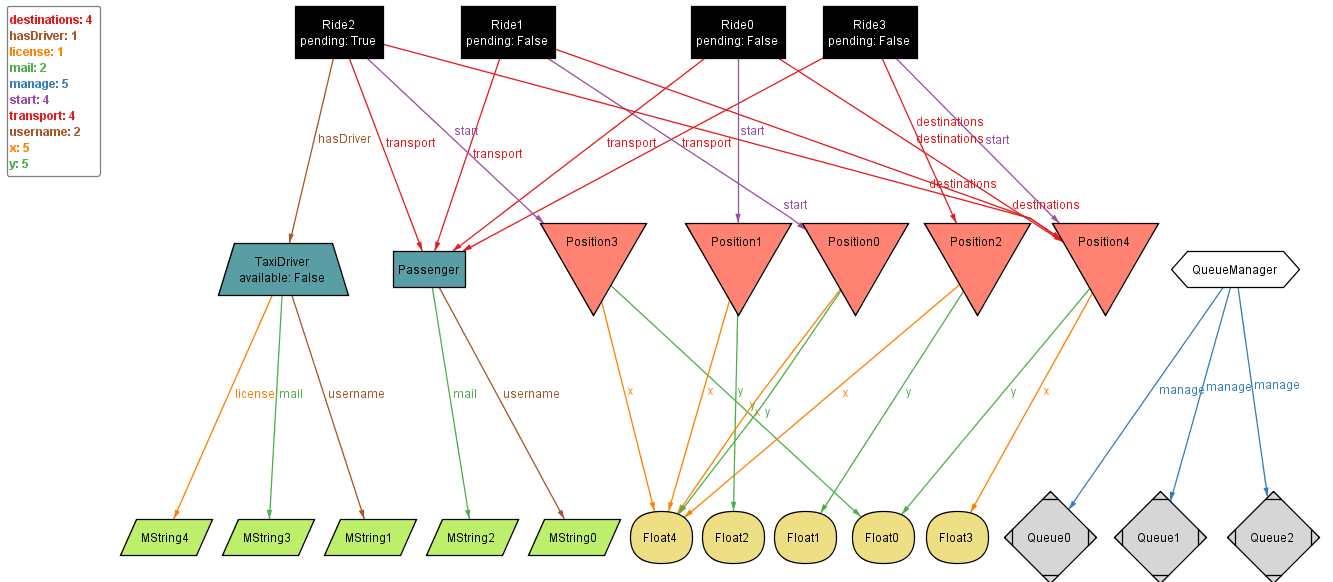
\includegraphics[angle=90,height=0.9\textheight]{world2}
\par\end{center}

\pagebreak{}


\subsection{Alloy metamodel}

The following platform metamodel was derived from the Alloy code in
section \ref{sub:Alloy-source-code} and is a further expansion of
the class diagram in section \ref{sub:Class-diagram}.

\begin{center}
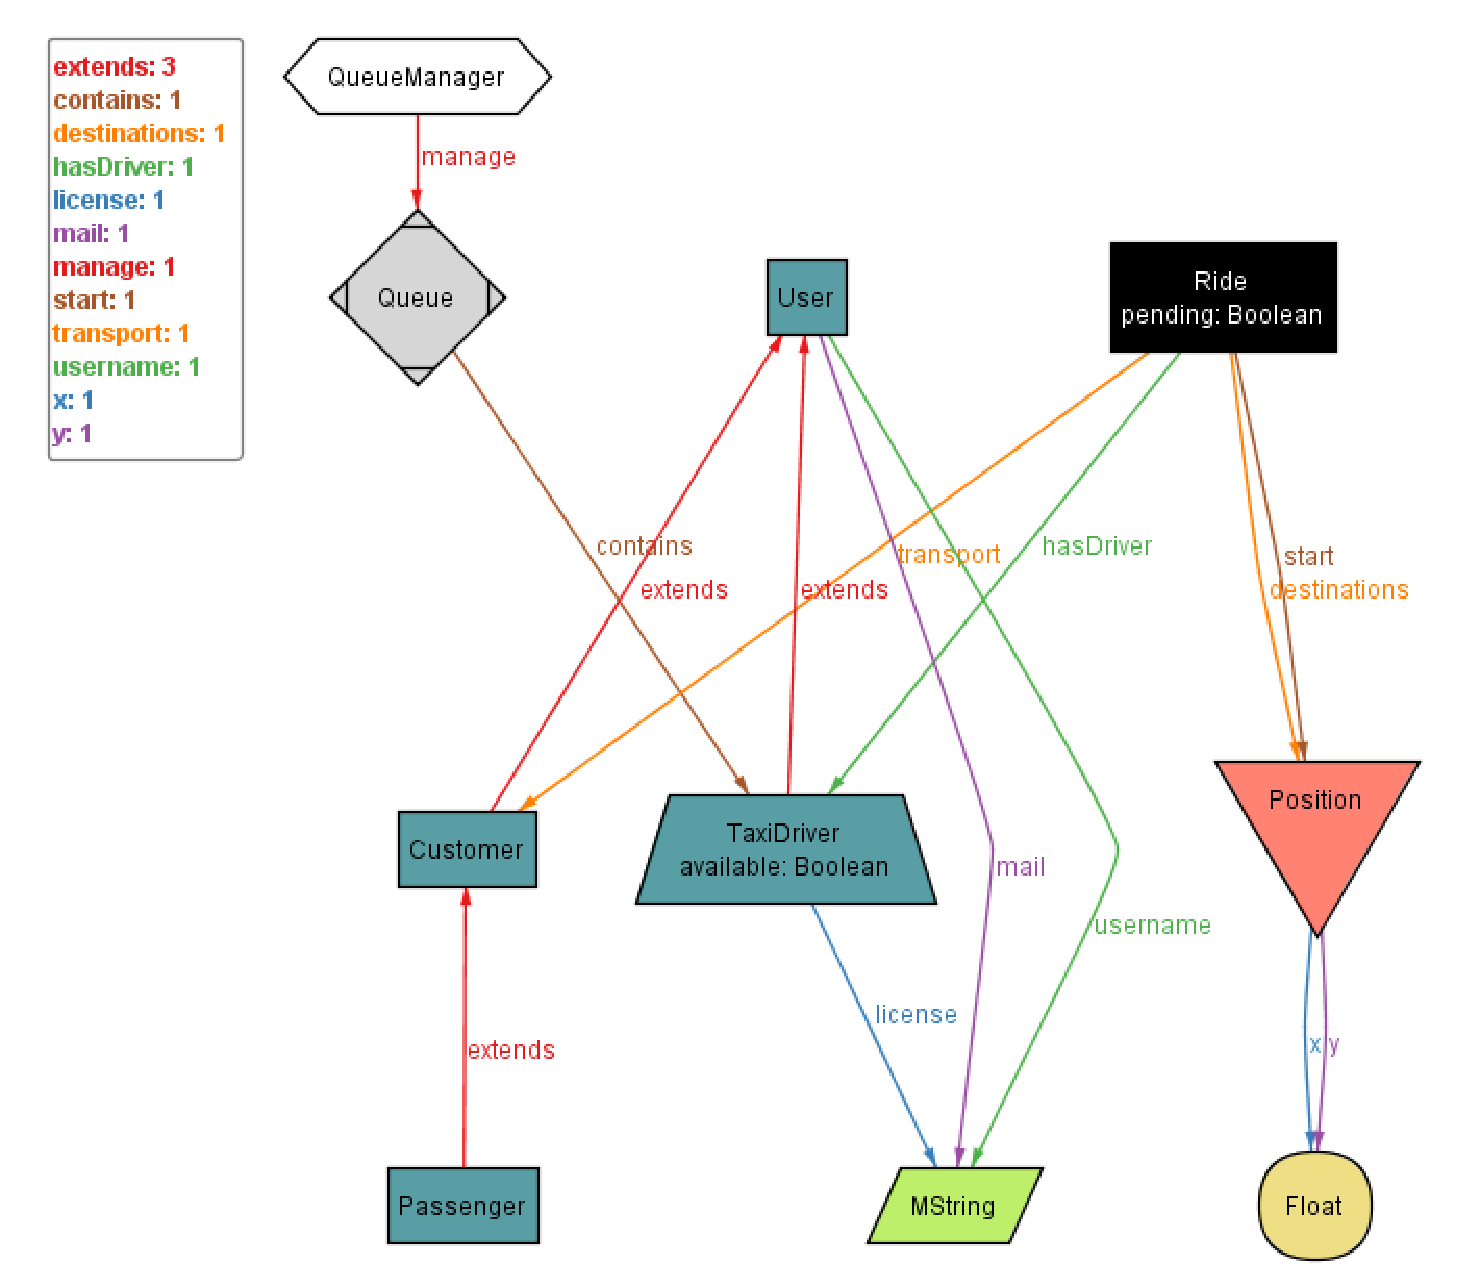
\includegraphics[width=1\textwidth]{Metamodel}
\par\end{center}

\pagebreak{}


\section{Additional Comments}

The production of this document has been a joint effort of all the
authors, with a fair distribution of the mansions which caused each
member of the group to work on all the parts of the document. 

The production has been carried out between 16/10/2015 and 6/11/2015
for a total time expense of: 
\begin{itemize}
\item \textbf{Group work}: 28 hours
\item \textbf{Individual work}:


\begin{tabular}{|c|c|}
\hline 
Daniele Grattarola (Mat. 853101) & 10.5 hours\tabularnewline
\hline 
Ilyas Inajjar (Mat. 790009)  & 9 hours\tabularnewline
\hline 
Andrea Lui (Mat. 850680) & 10 hours\tabularnewline
\hline 
\end{tabular}

\end{itemize}
\pagebreak{}
\end{document}
